In 2008, Del\'{e}glise et. al. \cite{Deleglise} performed markedly different state preparation and characterization compared to that done by Smithey et. al \cite{Smithey}. Their approach involved the use of a cavity quantum electrodynamics (QED) set-up. To prepare the initial state, a highly reflective mirror is brought to superconducting temperatures. The purpose of the mirror is to trap incident photons. One of the purposes of the low temperature for the mirror is to suppress spurious photons generated by the vacuum (which occurs with higher probablility - read: frequency - at higher temperatures. Their scheme purportedly traps the incident light between the mirrors for long times ($130 ms$). A stream of rubidium atoms are prepared such that the state of the atoms (rather the valence electrons) occupy the $n=50$ spherical orbital. The adjacent transition in this atom is the $n=51$ spherical orbital. These serve as the ground and first excited states.

The effect of the cavity field, C in figure \ref{DelSetUp}, on the stream of rubidium atoms is determined by a measurement of the field after the atom is determined to be in the ground or excited state (at D in figure \ref{DelSetUp}). Then, after the state of the atoms (whose state has been modified by the various fields) has been measured a sufficient number of times (millions) the density matrix for the field can be determined. The density matrix obtained for a variety of prepared states is show in figure \ref{DelMeasurements}. The focus of this paper was on the preparation of Schr\"odinger cat states, which are of the form : $|A|(\ket{\alpha}\pm\ket{-\alpha})$, where $|A|$ is the normalization constant and $\ket{\alpha}$ is the conventional notation for a coherent state of light. The reader is reminded that a coherent state of light is one that is expressed in the Fock (number) basis as : $\ket{a} = \sum_{n=0}^{\infty} e^{-\frac{1}{2}\alpha\alpha^*}\frac{\alpha^n}{\sqrt{n!}}\ket{n}=e^{-\frac{1}{2}\alpha\alpha^*}e^{\alpha\hat{a}^\dagger}\ket{0}$. The even cat states and the odd cat states are physically interesting in that an even cat state contains only Fock states of even value while an odd cat state contains only Fock states of odd value.

\begin{figure}%
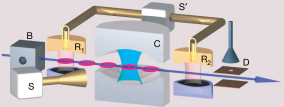
\includegraphics[width=284px,height=107px]{Figures/DelegliseSetUp.png}%
\caption{Cartoon of the experimental set-up used by Del\'{e}glise et. al. The Rydberg atoms (rubidium) are reported as being prepared in `Box B'. These are collimated from the exit port of Box B and projected through the cavity resonator at a speed of 250 $\frac{m}{s}$. Note that, though, there are two cavities external to the main central cavity, C. These cavities $R_1$ and $R_2$ are both used along with an external electromagnetic source (microwave) to prepare the Rydberg atoms in superposition states $\frac{1}{\sqrt{2}}\big(\ket{0}+e^{i\phi}\ket{1}\big)$. The state of the atoms once they have traveled through the three cavity resonators (and having been irradiated three separate times) is determined by the atomic detector, D. Note that the insets have been generated by taking the experimental nonlinearaties of the apparatuses into account.}
\label{DelSetUp}
\end{figure}

Now, while the state preparation is not explained in great detail, the authors of the Del\'eglise paper indicate that the state of the atom upon exiting the third cavity is a linear combination of an even photonic cat state and odd cat state. The even cat state is entangled with the ground state of the rubidium atom and the odd cat state is entangled with the excited state of the rubidium atom. Thus, detector D, which discriminates between excited and ground states of the rubidium atom, projects the state of the field onto one of the Schr\"odinger cat states. If the atom is detected without using detector D to measure the excitation of the atom, the state of the atom entangled to the coherent light in the resonator is, in this case, a statistical mixture of an even and odd cat state. Note that the measured quantity is the radiation escaping from cavity C (not the state of the atoms). The atoms are just used for projective purposes.

The tomography of the states is done in such a way as to, initially, obtain the density matrix of the system. Then, the Wigner function over the phase space (the real and imaginary parts of the field amplitude $\alpha$) is given by $W(\alpha)=\frac{2}{\pi}Tr[D(-\alpha)\rho D(\alpha)e^{i\pi N}]$, where the $N$ in the exponential is the standard bosonic number operator $N = a^\dagger a$. For obvious reasons, this exponentiated operator is often called the parity operator and has eigenvalues $(-1)^n$ (where n is the nth Fock state). The authors make note that the Wigner function would be experimentally determined if the ``atom-field phase shift'' was linear. I understand this to mean than nonlinearities in the mechanisms used to correlate the state of the atom (qubit) to that of the light make a direct determination of the Wigner function impossible. The results of measurement, post-processed, are shown in figure \ref{DelMeasurements}. The density matrices are not shown out of their irrelevance to this paper.

%As a minor addendum	 to the paper, the authors note the significance of the cat states to the study of decoherence. However, the necessity of using cat states (as opposed to any other special quantum state, was not justified.

\begin{figure}%
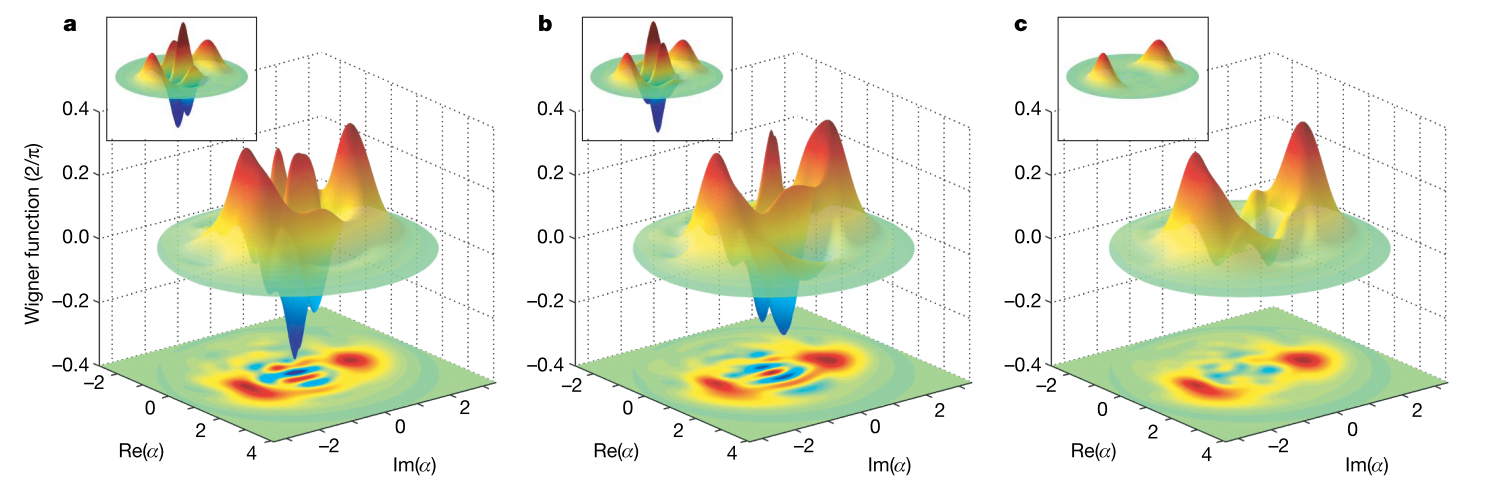
\includegraphics[width=440px,height=149px]{Figures/DelMeasurements.png}%
\caption{Shown in panels a), b) and c) are Wigner function reconstructions for three different states: a) An even Schr\"odinger cat state, b) an odd Schr\"odinger cat stat and c) a symmetric mixture of the even and odd cat states. The theoretically-predicted Wigner function for each respective state is given in the inset of each panel.}%
\label{DelMeasurements}%
\end{figure}

